\documentclass[pdftex,12pt,a4paper]{article}
\usepackage[pdftex]{graphicx}
\usepackage{xcolor}
\usepackage{marginnote}
\usepackage{enumitem}
\usepackage[hidelinks]{hyperref}
\usepackage[bottom=1.5cm, outer=5cm, inner=2cm, heightrounded,
marginparwidth=4cm, marginparsep=0.5cm]{geometry}

\begin{document}
    % Custom title page
    \begin{titlepage}
        \begin{center}
            
\includegraphics[width=5cm]{figures/kulogo}\\[1cm]
            {\Large \bfseries
                Spring 2014\\
                Computer Networks\\
                CMPE323\\[1cm]
            }
            {\large \bfseries
                \noindent Laboratory Experiment No. 9: Introduction to Dynamic
                Routing Protocols\\[1cm]
            }
        \end{center}

        \noindent \textbf{Aims and Objectives:}
            \begin{itemize}[leftmargin=4cm]
                \item Introducing dynamic routing protocols by studying basics
                    of Routing Information Protocol (RIP) version 2.
            \end{itemize}
            \vspace{0.5cm}

        \noindent \textbf{Materials Required:}
            \begin{itemize}[leftmargin=4cm]
                \item IP routers,
                \item PCs with Ethernet adapters,
                \item and straight-through/crossover/rollover cables.
            \end{itemize}
            \vspace{0.5cm}

        \noindent \textbf{Change Log:}
            \begin{itemize}[leftmargin=4cm]
                \item 15-5-2014: original document -- mkhonji.
                \item 16-5-2014: more coverage of the RIPv2 timers, replaced 
                    network merge by a single readily merged network -- mkhonji.
            \end{itemize}
    \end{titlepage}
    \newpage

    % Lab script content
    \section{Introduction}
        Consider a scenario where routers $R_1, R_2, \ldots R_n$ are
        interconnected using some partial mesh topology. If full end-to-end
        reachability is needed, then configuring static routing tables can
        have an high maintenance overhead. E.g. you may have to update the
        routing table configuration of all of the $n$ routers should you desire
        to add a new network that is reachable by all.

        While static routes are highly successful in limited scenarios, they
        can introduce maintenance challenges in larger networks as changes
        occur.

        Dynamic routing protocols address that problem: instead of using a
        human administrator to manually configure the routers $R_1 \ldots R_n$
        every time a new network is added, dynamic routing protocols allow us
        to configure the routers once such that they can dynamically
        communicate with themselves and learn the routing table automatically.
        Additionally, if there is a failure, dynamic routing protocols can
        allow for automatic self-healing by automatically choosing the next best
        path. 

        This lab covers a simple but widely spread routing protocol, namely
        Routing Information Protocol v2. The main changes in the 2$^{nd}$
        version is the addition of CIDR support (by adding subnet masks),
        authentication, multicasting communication instead of broadcasting,
        addition of requests,  route tags.

        While there are more scalable routing protocols, such as IS-IS and
        OSPF, RIPv2 remains fairly attractive as it has a very small overhead
        in \emph{small} networks.

        The work flow of RIPv2 is generally as follows (a lossy summary from
        RFC2453 for simplicity):
        \begin{itemize}
            \item RIPv2 is enabled on router interfaces, which allows their
                corresponding networks to be included in the RIPv2
                advertisements.
            \item Every interface that has RIPv2 enabled, sends RIPv2 messages
                that advertise its routing table every 30 seconds by default.
            \item Neighboring routers that hear such advertised
                RIP updates generally install them into their own routing table
                if the advertised networks have a better \emph{metric} than the
                one that is in the routing table (if there is any).
            \item A better metric by RIPv2 is simply the total number of layer
                3 hops that lead to a given network. 
                
                E.g. if $R_1$ is directly connected to network $N_1$, it shall
                advertise it to is neighboring routers while associating such
                network advertisement with a metric of 1 (as there are 1
                layer-3 hops). 
                
                Then, the receiving neighboring router (if any) will increment the hop
                count by 1 and then advertise it to its own neighbors (except
                the network from which the advertisement came from).

                This way, as the advertised network crosses more layer 3 hops,
                the metric will increase. By default, the maximum reachable metric is just
                15 hops. 
                
                A hop of 16 is possible but means ``infinity'' and is used to
                advertise lack of network reachability.
        \end{itemize}

        The RIPv2 protocol is structured as follows in Figures
        \ref{fig:ripoverview} and \ref{fig:ripentries}:
        \begin{figure}[tbh]
            \centering
            \begin{verbatim} 0                   1                   2                   3
 0 1 2 3 4 5 6 7 8 9 0 1 2 3 4 5 6 7 8 9 0 1 2 3 4 5 6 7 8 9 0 1
+-+-+-+-+-+-+-+-+-+-+-+-+-+-+-+-+-+-+-+-+-+-+-+-+-+-+-+-+-+-+-+-+
|  command (1)  |  version (1)  |       must be zero (2)        |
+---------------+---------------+-------------------------------+
|                                                               |
~                         RIP Entry (20)                        ~
|                                                               |
+---------------+---------------+---------------+---------------+\end{verbatim}
            \caption{RIPv2 message format. Note the possibility adding multiple
            routing advertisement entries --- Source RFC2453.}
            \label{fig:ripoverview}
        \end{figure}

        \begin{figure}[tbh]
            \centering
            \begin{verbatim} 0                   1                   2                   3 3
 0 1 2 3 4 5 6 7 8 9 0 1 2 3 4 5 6 7 8 9 0 1 2 3 4 5 6 7 8 9 0 1
+-+-+-+-+-+-+-+-+-+-+-+-+-+-+-+-+-+-+-+-+-+-+-+-+-+-+-+-+-+-+-+-+
| Address Family Identifier (2) |        Route Tag (2)          |
+-------------------------------+-------------------------------+
|                         IP Address (4)                        |
+---------------------------------------------------------------+
|                         Subnet Mask (4)                       |
+---------------------------------------------------------------+
|                         Next Hop (4)                          |
+---------------------------------------------------------------+
|                         Metric (4)                            |
+---------------------------------------------------------------+\end{verbatim}
            \caption{RIPv2 routing entry format --- Source RFC2453.}
            \label{fig:ripentries}
        \end{figure}

        Fields are:
        \begin{itemize}
            \item Command --- type of action (request(1) or response(2)).
            \item Version --- the version of RIP (1 for v1, and 2 for v2).
            \item Address Family ID --- the ID of the address family (2 for
                IPv4).
            \item Route tag --- this is helpful to group RIP advertisements for
                different treatments later one. However this is beyond the
                scope of this lab.
            \item IP address --- the IPv4 address of the advertised network.
            \item Subnet mask --- the subnet mask of the advertised network.
            \item Next hop --- the IP address of the gateway that packets
                to the network should be forwarded to. A next-hop of
                \texttt{0.0.0.0} is simply a self-reference of the interface of
                the advertising router.
            \item Metric --- the total number of hops that are to be crossed in
                order to reach the advertised network.
        \end{itemize}

        RIPv2 has the following timers as implemented by Cisco's IOS:
        \begin{itemize}
            \item Time interval between the updates $t_u$ --- by default, this timer
                is set to 30 seconds which causes the router to advertise routes from
                its routing table to its neighbors once every 30 seconds.
            \item Invalidation timer $t_i$ --- if a router does not receive a
                RIPv2 update about a given network for $t_i$ seconds, it will
                consider the network as unreachable, remove it from its routing
                table, and send RIPv2 messages that indicate the lack of
                reachability for such network. Lack of reachability in RIPv2 is
                advertised similar to normal network advertisements except for
                settting metric to 16. By default, $t_i = t_u \times 6 = 180$.
            \item Holddown timer $t_h$ -- this is a Cisco-specific extension
                that forbids the router from updating its routing table with
                better routes with regards to some given network for $t_h$
                seconds should the network get advertised as
                \emph{unreachable}. This is intended to minimize number of
                routing table updates in cases where too-frequent updates occur
                (e.g. fluctuating
                links)\footnote{\url{http://www.cisco.com/web/techdoc/dc/reference/cli/nxos/commands/rip/timers\_basic.html}}.
                By default, $t_h = 180$ seconds.
            \item Flush timer $t_f$ --- if a router does not receive a
                RIPv2 update about a given network for $t_f$ seconds, it will
                completely remove it from its routing table. By default, $t_i = 240$.
        \end{itemize}


    \section{Lab Preparation}
        \begin{enumerate}
            \item Connect a PC to the routers console port using a rollover
                cable\footnote{If using Linux: \texttt{screen /dev/ttySx} were
                \texttt{x} is the
                serial interfaces ID that is connected to the console
                cable. If using Windows: Use Hyperterminal or Putty to
                connect to \texttt{COMx} ports.}.
            \item Erase the configuration of the
                routers\footnote{\texttt{enable}, \texttt{erase
                startup-config}, \texttt{reload}, and make sure to answer
                \texttt{no} to all yes/no questions while hitting
                \emph{enter} for all \texttt{confirm} prompts.}.
            \item Connect a PC to the switches console ports using rollover
                cables.
            \item Erase the configuration of the
                switch\footnote{\texttt{enable}, \texttt{erase startup-config},
                \texttt{delete vlan.dat}, \texttt{reload}, and answer
                \texttt{no} to all yes/no questions while hitting \emph{enter}
                for all \texttt{confirm} prompts.}. \textbf{Note:} the switches are
                optional at this stage and can be omitted.
            \item Physically connect the lab as depicted in Figure \ref{fig:labtop}.
            \item Logically assign\footnote{For Linux \texttt{ifconfig eth0
                <ip\_addr>/<netmask\_bits>}, and for Cisco IOS \texttt{enable, config terminal,
            interface <interface\_ID>, ip address <ip\_addr> <netmask>, no
    shutdown}.} the following IP addresses and subnet masks:
                \begin{itemize}
                    \item R1's Gi0/1: 10.0.1.1/24
                    \item PC1's eth0: 10.0.1.2/24
                    \item R1's Gi0/0: 10.0.12.1/24
                    \item R2's Gi0/0: 10.0.12.2/24
                    \item R2's Gi0/1: 10.0.2.1/24
                    \item PC2's eth0: 10.0.2.2/24
                \end{itemize}
            \item Run Wireshark on all involved lab PCs as depicted in Figure
                \ref{fig:labtop}.
        \end{enumerate}

        \begin{figure}[tbh]
            \centering
            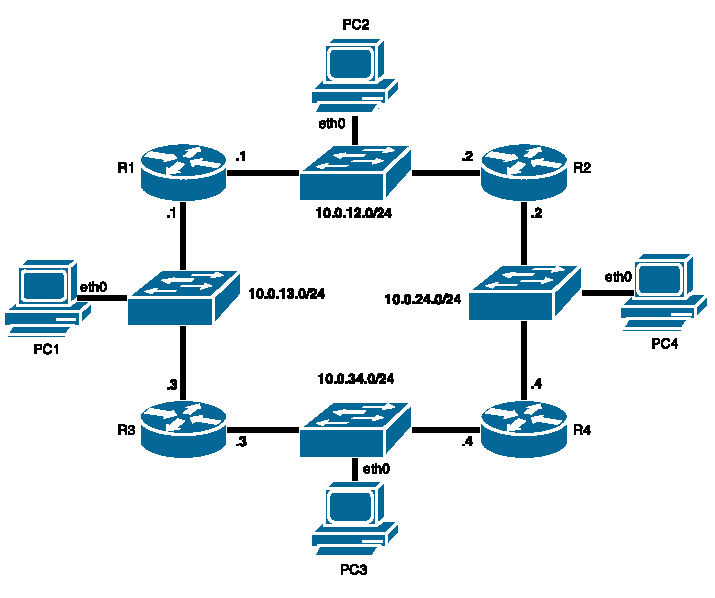
\includegraphics[width=0.9\textwidth]{figures/rip}
            \caption{Physical lab topology.}
            \label{fig:labtop}
        \end{figure}

    \section{Lab experiments}
        \subsection{Configuring RIPv2}
            Enable RIPv2 on all of the routers' interfaces and networks as follows:
            \begin{enumerate}
                \item \texttt{enable}.
                \item \texttt{config terminal}.
                \item \texttt{router rip}.
                \item \texttt{version 2}.
                \item \texttt{network 0.0.0.0}\footnote{This will activate
                    RIPv2 on all interfaces whose IP addresses fall under any
                    network as well as including their network IP addresses in the
                    RIPv2 advertisements.}
            \end{enumerate}

        \subsection{Verifying RIPv2}
            \begin{flushright}
                \textbf{[20 points]}\marginnote{\small \textbf{Note:} when done, show your
                work to the lab engineer for grading purposes.}
            \end{flushright}

            Verify the correctness of the configuration:
            \begin{itemize}
                \item \texttt{show ip protocols}.
                \item \texttt{show ip route}.
                \item Use the \texttt{ping} command to test the reachability.
            \end{itemize}

        \subsection{Analysis of converged RIPv2}
            \begin{flushright}
                \textbf{[30 points]}\marginnote{\small \textbf{Note:} when done, show your
                work to the lab engineer for grading purposes.}
            \end{flushright}

            While monitoring Wireshark instances on relevant PCs, answer
            the following questions:
            \begin{enumerate}
                \item What is the inter-RIPv2 update gap in seconds in average? How
                    does this time compare against the output from \texttt{show
                    ip protocols}?
                \item What are the networks and their
                    corresponding metrics as advertised by RIPv2:
                    \begin{itemize}
                        \item From R1 to R2?
                        \item From R1 to R3?
                        \item From R2 to R1?
                        \item From R2 to R2?
                        \item From R3 to R1?
                        \item From R3 to R4?
                        \item From R4 to R2?
                        \item From R4 to R3?
                    \end{itemize}
                \item What are the networks that are \emph{not} advertised:
                    \begin{itemize}
                        \item From R1 to R2?
                        \item From R1 to R3?
                        \item From R2 to R1?
                        \item From R2 to R2?
                        \item From R3 to R1?
                        \item From R3 to R4?
                        \item From R4 to R2?
                        \item From R4 to R3?
                    \end{itemize}
                \item What is the effect of advertising next-hop address of
                    \texttt{0.0.0.0} in the RIPv2 updates? You can use the
                    Linux command \texttt{traceroute} and the Cisco IOS command
                    \texttt{show ip route} as tools to answer this question.
                \item How do your previous answers correlate with the output of
                    Cisco IOS command \texttt{show ip route}.
            \end{enumerate}

        \subsection{Analysis of converging RIPv2}
            \begin{flushright}
                \textbf{[50 points]}\marginnote{\small \textbf{Note:} when done, show your
                work to the lab engineer for grading purposes.}
            \end{flushright}

            \begin{enumerate}
                \item Shutdown the router R1, change PC1's default gateway to
                    point to R3, and while keeping an eye on
                    Wireshark instances, answer the following:
                    \begin{itemize}
                        \item Find which PCs cannot successfully ping which other PCs?
                        \item For those PCs that cannot successfully ping some
                            other PCs, how long did it take the routers (using
                            RIPv2) to converge on the alternative routing
                            setup? Compare this time against those timers in
                            Cisco's IOS command \texttt{show ip protocols}.
                        \item Analyze the captured RIPv2 packets on the
                            Wireshark instances and describe the change that
                            occurred in the content of the RIPv2 messages and
                            how that facilitated the convergence of the network
                            to accommodate the fallen router.
                    \end{itemize}
            \end{enumerate}

        \subsection{Extra questions (not graded)}
            \begin{itemize}
                \item Inject a spoofed RIPv2 packet such that  you either cause a
                    DoS or a MitM attack. Using \texttt{macframesender-v2.c} is
                    easy as it calculates the IP checksum for you automatically
                    and the UDP checksum can be disabled by setting its value
                    to \texttt{0x0000}.

                    The basic idea is using your PC to advertise reachability
                    to a network with a much lower metric than the other
                    routers.

                    If a router receives such advertisement while setting
                    yourself as the next-hop, and if your metric is lower than
                    any other advertisement that the router has heard to so
                    far, the router will update its routing table and start
                    forwarding traffic of that network to your PC instead!
                    It's up to you to make a DoS (by dropping them) or a MitM
                    (by re-routing them while observing them or modifying
                    them).

                \item Logically thinking, list some solutions that, if applied,
                    the above MitM attack would become much harder to happen.
            \end{itemize}
    \appendix
    \section{Relevant protocols}
                \begin{figure}[tbh]
                    \centering
                    \begin{verbatim} 0                   1                   2                   3
 0 1 2 3 4 5 6 7 8 9 0 1 2 3 4 5 6 7 8 9 0 1 2 3 4 5 6 7 8 9 0 1
+-+-+-+-+-+-+-+-+-+-+-+-+-+-+-+-+-+-+-+-+-+-+-+-+-+-+-+-+-+-+-+-+
|Version|  IHL  |Type of Service|          Total Length         |
+-+-+-+-+-+-+-+-+-+-+-+-+-+-+-+-+-+-+-+-+-+-+-+-+-+-+-+-+-+-+-+-+
|         Identification        |Flags|      Fragment Offset    |
+-+-+-+-+-+-+-+-+-+-+-+-+-+-+-+-+-+-+-+-+-+-+-+-+-+-+-+-+-+-+-+-+
|  Time to Live |    Protocol   |         Header Checksum       |
+-+-+-+-+-+-+-+-+-+-+-+-+-+-+-+-+-+-+-+-+-+-+-+-+-+-+-+-+-+-+-+-+
|                       Source Address                          |
+-+-+-+-+-+-+-+-+-+-+-+-+-+-+-+-+-+-+-+-+-+-+-+-+-+-+-+-+-+-+-+-+
|                    Destination Address                        |
+-+-+-+-+-+-+-+-+-+-+-+-+-+-+-+-+-+-+-+-+-+-+-+-+-+-+-+-+-+-+-+-+
|                    Options                    |    Padding    |
+-+-+-+-+-+-+-+-+-+-+-+-+-+-+-+-+-+-+-+-+-+-+-+-+-+-+-+-+-+-+-+-+\end{verbatim}
                    \caption{Internet Protocol (IP) version 4 header format --- Source RFC791.}
                    \label{fig:ipv4}
                \end{figure}

        \begin{figure}[tbh]
                    \begin{center}
                    \begin{verbatim}
               0      7 8     15 16    23 24    31
               +--------+--------+--------+--------+
               | Source Port     | Destination Port|
               +--------+--------+--------+--------+
               |     Length      |    Checksum     |
               +--------+--------+--------+--------+
               |          data octets ...
               +---------------- ...\end{verbatim}
            \end{center}
            \vspace{-15pt}
            \caption{UDP Header Format --- Source: RFC768.}
            \label{fig:udp}
            \vspace{10pt}
        \end{figure}

\end{document}
